%%%%%%%%%%%%%%%%%%%%%%%%%%%%%%%%%%%%%%%%%%%%%%%%%%%%%%%%%%%%%%%%%%%%%%%%%%%%%%%%%%%%%%%%%%%%%%%%%%%
% Chapter 3 -> Single Multimodal Integration Problem
% Author: Mingbo Cheng
%%%%%%%%%%%%%%%%%%%%%%%%%%%%%%%%%%%%%%%%%%%%%%%%%%%%%%%%%%%%%%%%%%%%%%%%%%%%%%%%%%%%%%%%%%%%%%%%%%%
%\addbibresource{~/MEGA/MEGAsync/phd/thesis_Cheng/preamble/thesis.bib}
%\addbibresource{/home/mingbo/MEGAsync/phd/thesis_Cheng/preamble/thesis.bib}
\chapter{Single Cell Multimodal Integration Problem}
\label{chapter:problem_inte}
\graphicspath{{chapter3/figs/}}

\subsection{Single Cell Multimodal Integration}
We will discuss the computational challenge of integrating single-cell multimodal data, provide an overview of current methods for the task, and outline our objectives for addressing the limitations present in existing computational approaches to single-cell multimodal integration.
\subsubsection{Challenge of Single Cell Multimodal Integration}
\label{background:sec2:challenge_integration}
Single-cell multimodal profiling represents a nascent field, and the integration of single-cell multimodal data, while several tools have been developed for this purpose, still poses challenges:

\begin{itemize}
	\item \textbf{Heterogeneous statistical properties:}
	Different modalities exhibit distinct statistical properties, presenting a challenge for the integration of single-cell multimodal data. For instance, the feature size of single-cell surface proteins is typically around 100, while single-cell RNA-seq and single-cell ATAC-seq have feature sizes of 20,000+ and 100,000+~(\fref{fig:modalities_differences}A). The sparsity levels of the feature matrices for different modalities also vary significantly. For example, there are more than 10\% non-zero entries for scRNA-seq data, whereas scATAC-seq data has less than 3\% non-zero entries~\citep{li2021chromatin}, and surface protein data has more than 70\% non-zero entries~(\fref{fig:modalities_differences}B). Moreover, the feature distributions significantly differ among distinct modalities~(\fref{fig:modalities_differences}C). The substantial differences between modalities present a significant challenge in deriving a unified latent space that effectively incorporates all features without losing valuable information.


	\item \textbf{Modality Compatibility:}
	Increasingly, new protocols are being developed to simultaneously measure features in the same single cell, such as open chromatin, gene expression, protein, and DNA methylation. The combinations of different modality types present a challenge for integration; Certain methods, such as scAI~\citep{jin2020scai}, are designed to handle only two modalities, while others, like Liger~\citep{kriebel2022uinmf}, are restricted to specific feature matrices.

	\item \textbf{Scalability:}
	As sequencing costs decrease and technologies improve, we anticipate that multimodal datasets will follow a similar trend as single-cell RNA sequencing~(scRNA-seq), where in less than ten years, the size of experiments increased from the order of tens to millions of cells~\citep{svensson2018exponential}. More efficient methods are needed, ones that require less memory and reduced running time.

	\item \textbf{Interpretability:}
	Interpretation of each component of the latent space is essential to understand the information it captured in the latent space, some methods like Seurat WNN~\citep{hao2021seurat4} only delivered a network for the integration. When associating molecular features with the latent space, it's better if the method is capable of interpreting each component using features from specific modalities, and most methods lack this ability.

	\item \textbf{Removal of batch effects}:
	In single-cell multimodal integration, addressing heterogeneous features across different modalities is crucial, and the challenge extends to mitigating batch effects arising from both biological and technical sources. Certain methods, such as scAI~\citep{jin2020scai}, might be limited in their ability to incorporate external batch correction techniques, potentially leading to confounding results from combined batches and biological variations.

	\item \textbf{Validation}
	Evaluating the outcomes of data integration presents a significant challenge. In practice, there is no definitive ground truth, necessitating an evaluation based on downstream analysis tasks, such as assessing clustering agreement with true labels. However, these true labels, often annotations from a study, may introduce noise or inaccuracies in cell type identification. Therefore, a thorough validation should be applied to comprehensively assess the effectiveness of a method.

  \item \textbf{Execessive Presumption}
  Most methods either assume a specific data distribution or involve fitting the model with several parameters, requiring prior knowledge that may not be universally applicable. For example, Seurat WNN requires inputting the number of neighbors and scaling factor for the neighborhood, and MOFA involves several hyperparameters for model regularization, detection of number of factors and learning rates. Moreover, MOFA requires manual selection of informative components for downstream analysis after obtaining the latent components. A method is needed to automatically identify the most important shared information across different modalities.

\end{itemize}

\begin{figure}[!ht]
	\centering
	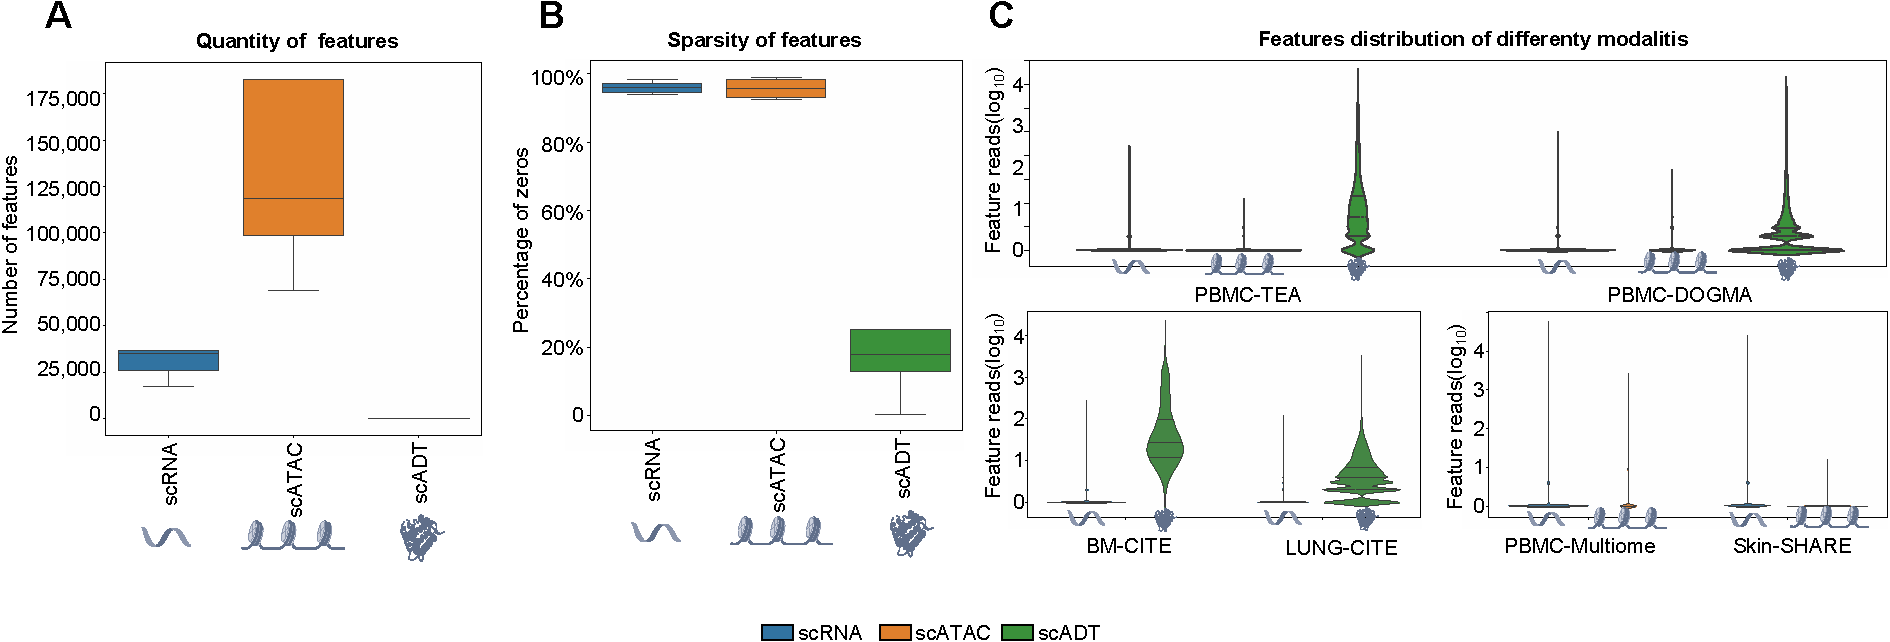
\includegraphics[width=0.95\textwidth]{feature_statistic/fig}
	\vspace{0.1cm}
	\caption[features characteristics comparison showing the challenge of multimodal integration.]{Illustration of six single-cell multimodal data. A) Number of features in scRNA, scATAC and scADT modalities. B) Percentage of zero entries in the three modalities, C) Element counts percentages in different modalities for the six single cell multimodal data.}
	\label{fig:modalities_differences}
\end{figure}

\subsubsection{Computational Methods for Single Cell Multimodal Integration}
\label{background:sec2:integration}
The challenges discussed in \sref{background:sec2:challenge_integration} regarding the integration of single-cell multimodal data pose difficulties in developing an efficient and effective integration method.

\begin{table}[!ht]
	\small
	\centering
	\begin{tabular}{llllll}
		\toprule
		Name & algorithm & modality types & \#modalities & Reference \\
		\midrule
    DIABLO & PLS-DA & universal & any & \cite{singh2019diablo}\\
    Liger & NMF & shared-features& 2 & \cite{kriebel2021nonnegative} \\
		MOFA   &  Matrix Factorization & universal & any &  \cite{argelaguet2020mofa+} \\
		Schema & Metrics learning  & universal & any & \cite{singh2021schema} \\
    scAI & Matrix Factorization & scRNA,scATAC & 2 & \cite{jin2020scai}\\
		Seurat WNN	 & WNN & universal & any & \cite{hao2021seurat4} \\
		\bottomrule
	\end{tabular}
	\vspace{0.1cm}
	\caption[Overview of computational integration methods]{Overview of computational integration methods.}
	\label{tab:methods_integration_overview}
\end{table}

Several methods have been developed to address this task, and we will now review the computational single-cell multimodal integration methods available in the literature. These methods can be classified into four groups based on the techniques they employ. The first group encompasses matrix factorization, which breaks down the multimodal count matrix into the product of two matrices. One matrix contains the latent factors representing the features, while the other incorporates the cells embedded in the latent factor space~(e.g., MOFA, scAI, Liger). The second group endeavors to construct a weighted nearest network that captures common information across all modalities~(e.g., Seurat WNN). The third group seeks to maximize the covariance or correlation between two modalities~(e.g., DIABLO, Symphony). The fourth group employs metric learning to reweigh modality features by maximizing their agreement with other modalities~(Schema). \tref{tab:methods_integration_overview} summarizes the characteristics of each method.
 \begin{figure}[!h]
  	\centering
  	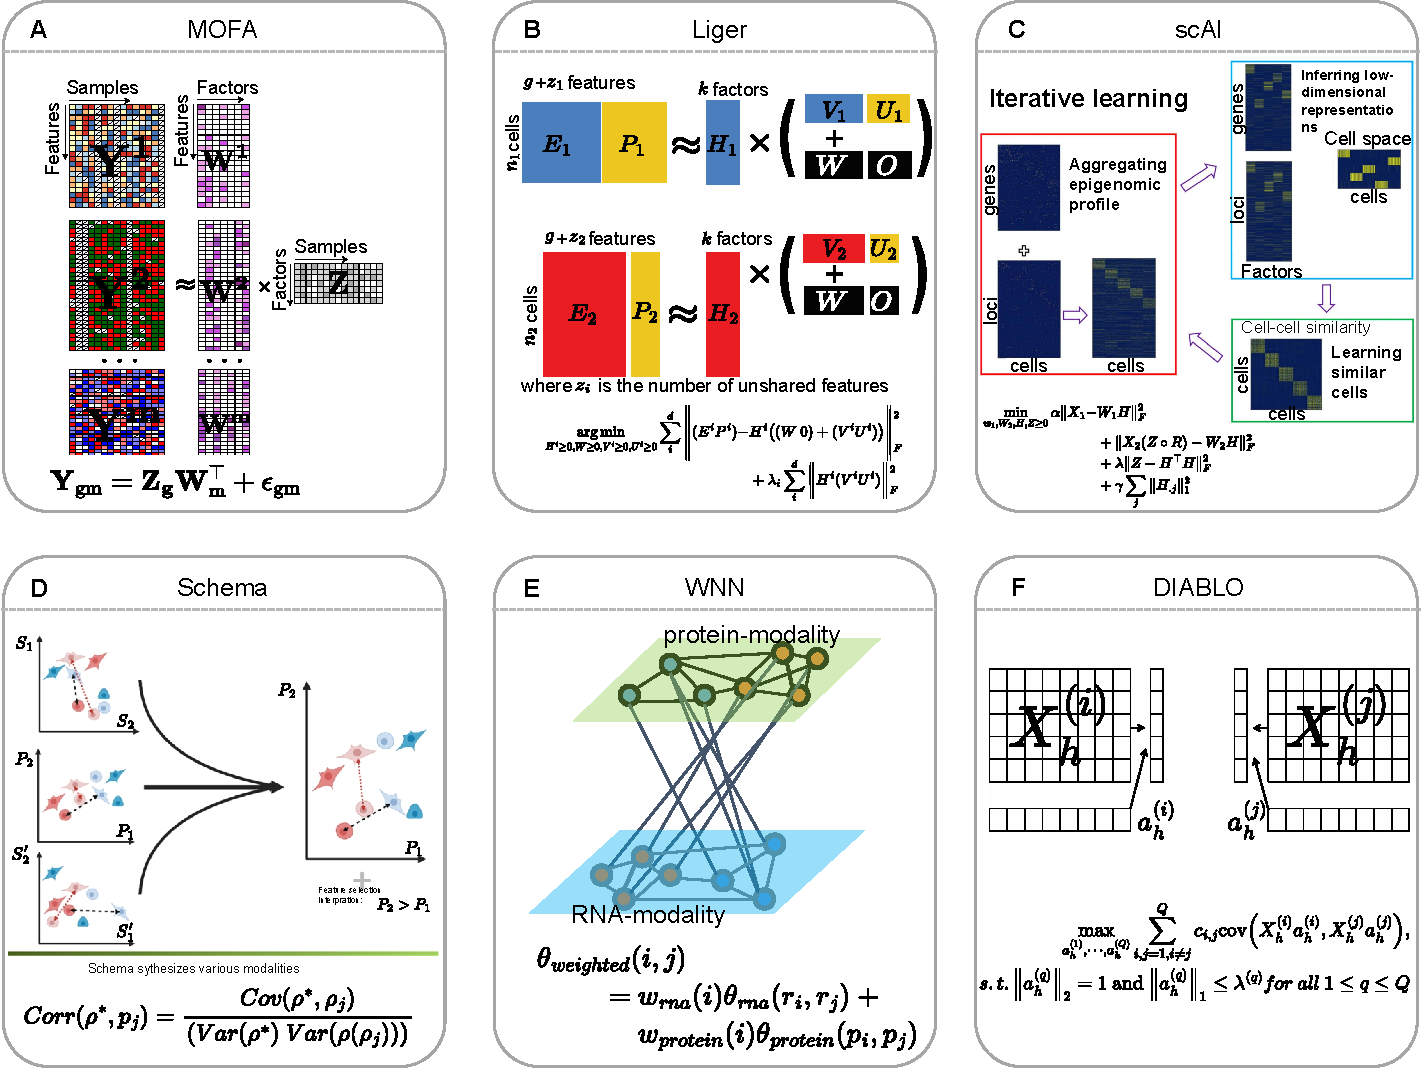
\includegraphics[width=0.9\textwidth]{Alg/fig}
  	\vspace{0.1cm}
  	\caption[Illustration of competing integration competing method.]{\textbf{Illustration of competing integration competing method.} \emph{Source~\cite{kriebel2022uinmf}}~(modified to fit thesis format and/or clarify key points)
  }
  	\label{fig:Alg}
 \end{figure}


\begin{description}
  \item[DIABLO]
  Data Integration Analysis for Biomarker discovery using Latent cOmponents~(DIABLO) is a generalization of sGCCA~\citep{tenenhaus2014variable}, which is a multivariate extension of canonical correlation analysis~(CCA). For $Q$ normalized and centered data matrices $X^1, \cdots, X^Q$ of dimensions $N\times D_q$, where $N$ denotes the number of cells and $D_q$ denotes the number of features. DIABLO aims to find a set of $H$ linear combinations of the $Q$ data matrices that are maximally correlated. The linear combinations are defined as:
  \begin{equation}
  \begin{aligned}
  	\underset{a_h^{(1)},\cdots,a_h^{(Q)}}{\max} \sum_{i,j=1, i\neq j}^Q c_{i,j} \text{cov}(X_h^{(i)} a_h^{(i)}, X_h^{(j)} a_h^{(j)}),\\
  	s.t. \|a_h^{(q)}\|_2 = 1, \text{ and } \|a_h^{(q)}\|_1 \leq \lambda^{(q)}, \text{for all} 1\leq q \leq Q.
  \end{aligned}
  \end{equation}
  Where $a_h^{(q)}$ is the variable coefficient vector for the $h$-th linear combination of the $q$-th data matrix, and $c_{i,j}$ is the weight of the correlation between the $i$-th and $j$-th data matrices. The first constraint is to normalize the linear combination, and the second constraint is to sparsify the linear combination. DIABLO solves the optimization problem by iteratively updating the $a_h^{(q)}$ and $c_{i,j}$ until convergence.


 \begin{figure}[!h]
  	\centering
  	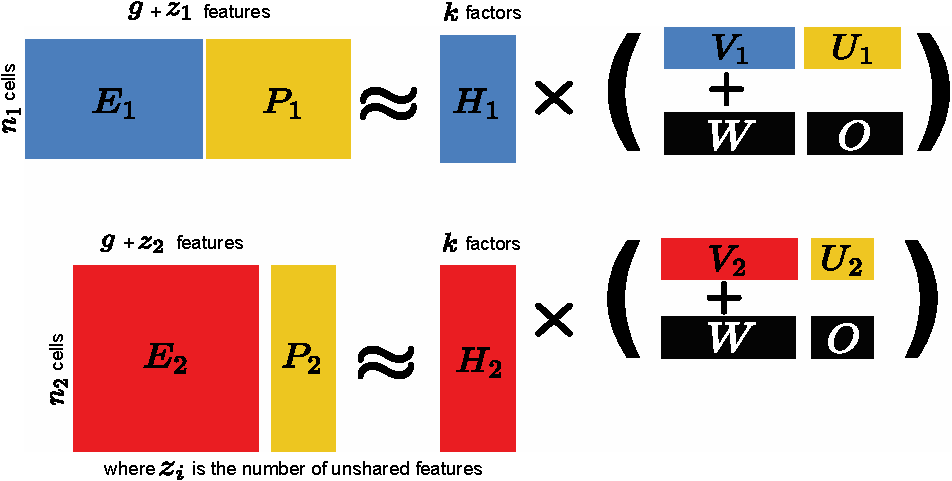
\includegraphics[width=0.6\textwidth]{Alg_Liger/fig}
  	\vspace{0.1cm}
  	\caption[Illustration of Liger integration competing method.]{\textbf{Illustration of Liger integration competing method.} Liger Schematic representation of the matrix factorization strategy~(top) and the formulation of the optimization problem~(bottom). The introduction of a factor matrix $U_i$ enables the utilization of unshared features in joint matrix factorization. Each dataset~($E_i$) undergoes decomposition into shared metagenes~($W$), dataset-specific metagenes constructed from shared features~($V_i$), unshared metagenes~($U_i$), and cell factor loadings~($H_i$). The inclusion of the U matrix enables unshared features occurring in only one dataset to contribute to the resulting integration. \emph{Source~\cite{kriebel2022uinmf}}~(modified to fit thesis format and/or clarify key points)
  }
  	\label{fig:Alg_Liger}
 \end{figure}

  \item[Liger]
  Linked Inference of Genomic Experimental Relationships~(Liger)~\citep{kriebel2022uinmf} implemented UINMF algorithm, which uses iterative Non-negative Matrix Factorization~(iNMF) to learn a common latent space across multiple modalities~(\fref{fig:Alg_Liger}). It allows the inclusion of both shared and unshared features across modalities to learn a common latent space. They incorporate intergenic peaks from snATAC-seq data and additional genes not measured in all datasets. For each data set $E^1, E^2, \cdots, E^n$, Liger first normalizes the data, and selects $m$ variable genes~(shared across all datasets), and $z_i$ variable features, such that after scaling $E^i \in R_{+}^{(m+z_i)\times n_i}\ (i=1,\cdots,N)$. Given $K$ and $\lambda_i$, the objective function is:
  \begin{equation}
	  \underset{H^i\geq 0,W\geq 0, V^i\geq 0, U^i \geq 0}{\arg\min} \sum_i^{d}\Big\| (E^i P^i) - H^i \big((W 0) + (V^i U^i)\big)\Big\|_{F}^2 + \lambda_i\sum_i^d\Big\|H^i(V^i U^i)\Big\|_{F}^2
  \end{equation}
  Liger uses coordinate block descent~(BCD) to solve the optimization problem, which derives the parameters into blocks and finds the optimal solution for each block iteratively.


\begin{figure}[!h]
  	\centering
  	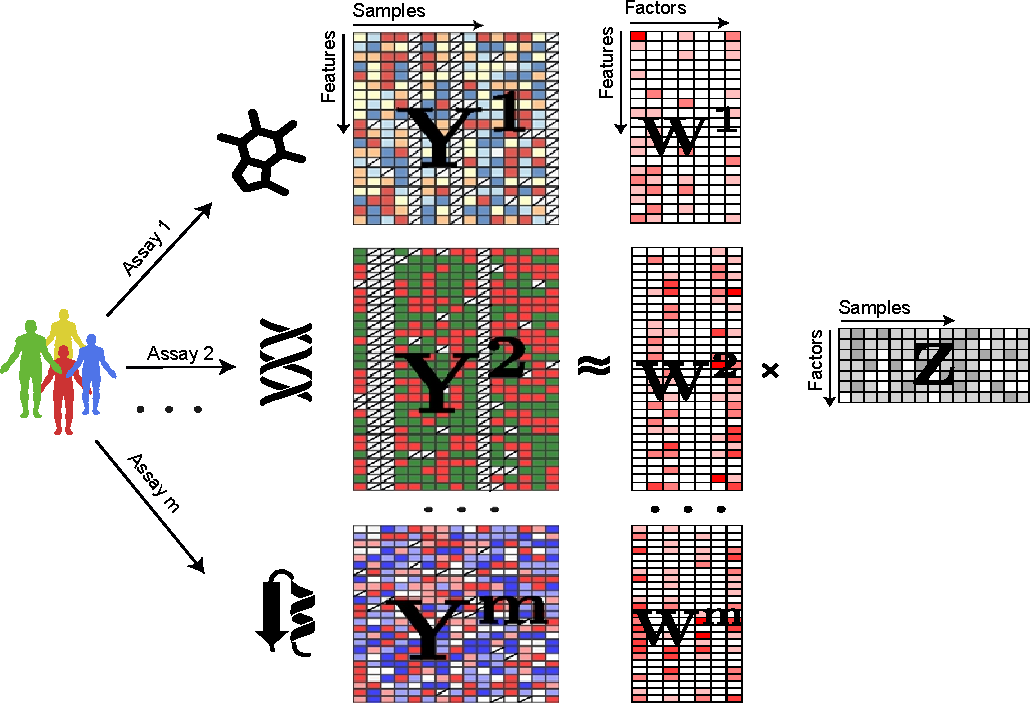
\includegraphics[width=0.65\textwidth]{Alg_MOFA/fig}
  	\vspace{0.1cm}
  	\caption[Illustration of MOFA integration competing method.]{\textbf{Illustration of MOFA integration competing method.} MOFA takes $m$ data matrices as input $Y_1, \cdots Y_m$, one or more from each data modality, with co-occurrent samples but features that are not necessarily related and that can differ in numbers. MOFA decomposes these matrices into a matrix of factors~($Z$) for each sample and $m$ weight matrices, one for each data modality~($W_1,\cdots, W_m$) where white cells in the weight matrices correspond to zeros~(i.e., inactive features). The cross symbol in the data matrices represents missing values. \emph{Source~\cite{tewari2017mofa}}~(modified to fit thesis format and/or clarify key points)
  }
  	\label{fig:Alg_MOFA}
\end{figure}
 
  \item[MOFA]
  Multi-Omics Factor Analysis+~(MOFA+)~\citep{argelaguet2020mofa+} uses Bayesian group factor analysis and variational inference to decompose individual modalities simultaneously by estimating a common latent factor matrix $Z$, as well as the weights for the transformation of the modalities to the latent space~(\fref{fig:Alg_MOFA}). MOFA+ includes a procedure to determine the optimal number of factors~(dimension of the latent space) and has several hyper parameters for model regularization, detection of number of factors and learning rates. Specifically, it decomposes simultaneous multimodal of $M$ data matrics $Y^1, \cdots, Y^M$ of dimensions $N\times D_m$, where $N$ denotes the number of cells and $D_m$ denotes the number of features, $G$ is the number of sample groups, and $N_g$ is the number of samples in the $g$th group and $K$ is the number of factors. The matrix decomposition is:
  \begin{equation}
  Y_{gm} = ZgW_m^{T} + \varepsilon_{gm},
  \end{equation}
  Where $Y_{gm}$ is the the matrix of observations for the $m$th data modality and the $g$th group, $Z_g$ is the matrix of latent factors for the $g$th group, $W_m$ is the matrix of weights for the $m$th data modality, and $\varepsilon_{gm}$ is the matrix of residuals. The latent factors $Z_g$ are shared across all modalities, while the weights $W_m$ are specific to each modality. %%TODO: the decomposition algorithm

\begin{figure}[!h]
  	\centering
  	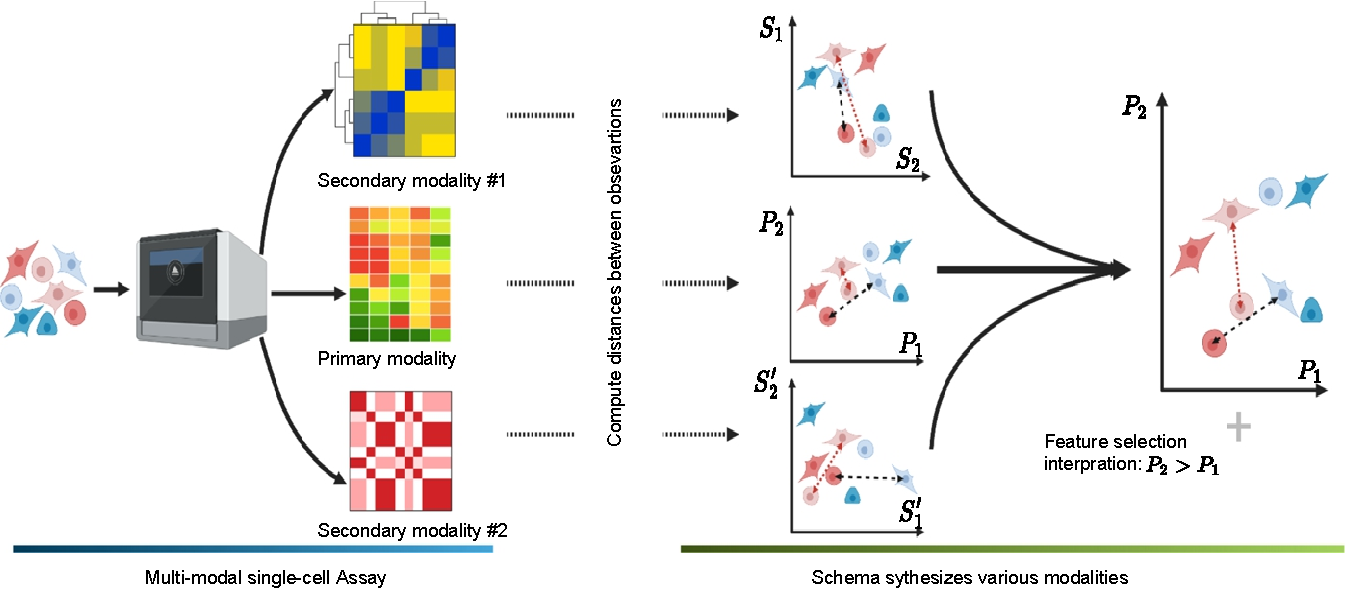
\includegraphics[width=0.8\textwidth]{Alg_Schema/fig}
  	\vspace{0.1cm}
  	\caption[Illustration of Schema integration competing method.]{\textbf{Illustration of Schema integration competing method.} Schema explores metrics learning to re-weigh modality features through maximizing the agreement with other modalities. Specifically, it utilizes quadratic programming~(QP) to learn a scaling transformation $u$ for the primary matrix $X$ such that pairwise distances of the transformation $u * x_i$~(where $*$ is coordinate-wise multiplication, for each $x_i\in X$) are highly correlated in other modalities. \emph{Source~\cite{singh2021schema}}~(modified to fit thesis format and/or clarify key points)
 } 
  	\label{fig:Alg_Schema}
\end{figure} 

  \item[Schema]
  Schema~\citep{singh2021schema} applied metrics learning to reweigh modality features by maximizing the agreement with other modalities~(\fref{fig:Alg_Schema}). Specifically, it utilizes quadratic programming~(QP) to learn a scaling transformation $u$ for the primary matrix $X$ such that pairwise distances of the transformation $u * x_i$~(where $*$ is coordinate-wise multiplication, for each $x_i\in X$) are highly correlated other modalities. Specifically, it assumes $N$ observations across $r$ datasets $D_j$, where $j=1,\cdots,r$ and $D_j = \{x_i^{j}: i = 1,2,\cdots,N\}$ contains data for each observation. First, it refers $D_1$ as the primary modality and $D_2,\cdots,D_r$ as the secondary modalities. Next, it computes the pairwise distances $\rho_1,\cdots,\rho_j$ for each modality $D_j$ where $\rho_j(x_n^{j}, x_m^{(j)})$ is the distance between observation $n$ and $m$ in $D_j$. Then, it aims to find a transformation $\Omega$ with $\Omega(D)$ generating a dataset $D^{*}$ such that the Euclidean metric $\rho^{*}$ on $D^{*}$ on $D^{*}$ aligns the various metrics. $\Omega$ is limited to be a scaling transformation $\Omega(D) = \{diag(u)x: x \in D\}$, where $u \in \mathbb{R}^{k}$ and $diag(u)$ is a $k\times k$ diagonal matrix with diagonal entries $u$. Then, the squared distance between points under the transformation is given by:
  \begin{equation}
  \rho^{*}(x_n, x_m) = \|diag(u)x_n - diag(u)x_m\|^2 = \|diag(w)(x_n - x_m)\|^2
  \end{equation}
  where $w$ is the element-wise square of u. The scaling transforms u acts as a feature-weighting mechanism to choose the features of $D_1$ that align the datasets best. Schema integrates between the metrics $\rho_j$ to learn a metric $\rho^{*}$ that aligns well with all of them. The correlation between $\rho^{*}$ and $\rho_j$ is measured by the Pearson correlation coefficient. And to tackle multiple modalities, Schema maximizes the sum of Pearson correlation between $\rho^{*}$ and all other modalities pairwise distances $\rho_2,\cdots,\rho_j$.
\begin{figure}[!h]
  	\centering
  	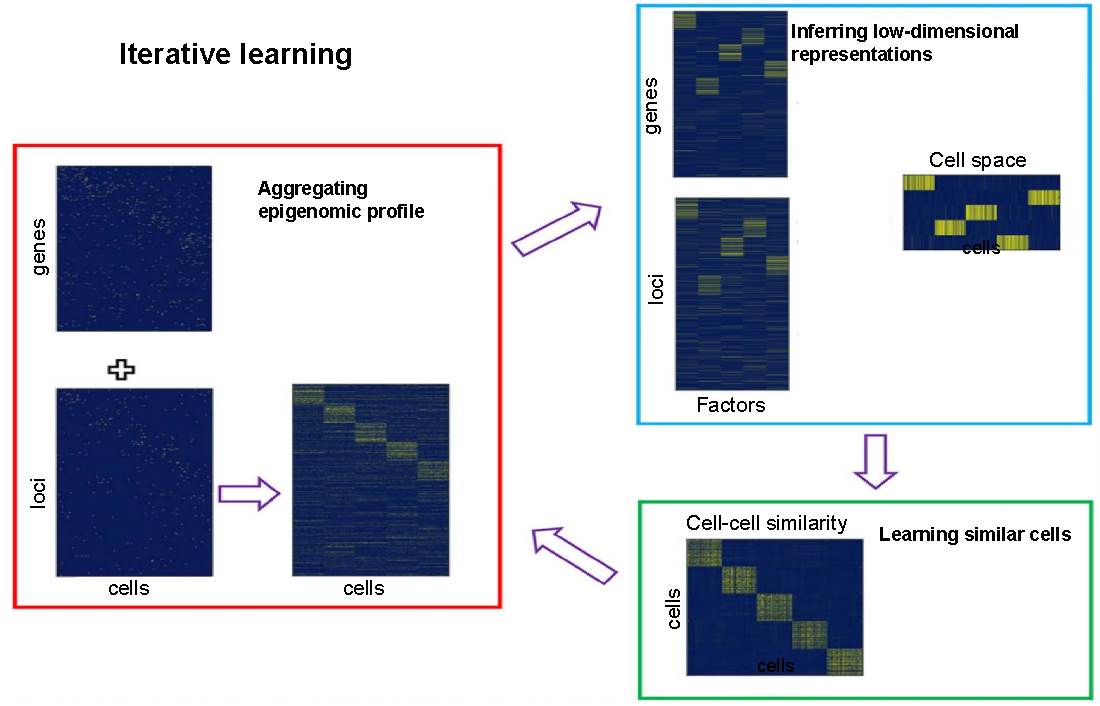
\includegraphics[width=0.55\textwidth]{Alg_scAI/fig}
  	\vspace{0.1cm}
  	\caption[Illustration of Seurat scAI integration competing method.]{\textbf{Illustration of Seurat scAI integration competing method.} scAI iteratively learns aggregated epigenomic profiles and low-dimensional representations from parallel scRNA-seq and scATAC-seq/single cell DNA methylation data. Input matrices consist of cells in rows and genes or loci in columns. The first step involves aggregating the epigenomic profile based on a randomly initiated cell-cell similarity matrix. In the second step, both transcriptomic and aggregated epigenomic data are concurrently decomposed into low-rank matrices, with gene, locus, and cell loading matrices indicating contributions for each factor. The third step computes a cell-cell similarity matrix based on the cell loading matrix. These steps iterate until a predefined stop criterion is met. \emph{Source~\cite{jin2020scai}}~(modified to fit thesis format and/or clarify key points)
  }
  	\label{fig:Alg_scAI}
\end{figure}

  \item[scAI]
  Single-cell Aggregation and Integration~(scAI)~\citep{jin2020scai} is aimed to integrate multiple modalities with different feature types specific for scRNA $(X_1\in \mathbb{R}^{p \textbf{ genes} \times n \textbf{ cells}})$ and scATAC/DNA methylation$~(X_2\in \mathbb{R}^{q \textbf{ loci}\times n \textbf{ cells}})$ modalities~(\fref{fig:Alg_scAI}). It creates a matrix factorization model:
  \begin{equation}
  \min_{w_1,W_2,H,Z\geq 0} \alpha \|X_1-W_1H\|_F^2 + \|X_2(Z \circ R)-W_2H\|_F^2 + \lambda \|Z-H^\top H\|_F^2 + \gamma\sum_j \|H_{.j}\|_1^2
  \end{equation}
  Where $W_1$ and $W_2$ are the gene loading and locus loading matrices with size $p\times K$ and $q\times K$($K$ is rank), respectively. Each of the $K$ columns is considered as a factor to capture a biological process/signal relating to a specific cell type. $W_1^{ik}$ and $W_2^{ik}$ are the loading values of gene $i$ and locus $i$ in factor $k$, and the loading values represent the contributions of gene $i$ and locus $i$ in factor k. $H$ is the cell loading matrix with size $K\times n$ ($H_{.j}$ is the $j$th column of $H$), and the entry $H^{kj}$ is the loading value of cell $j$ when mapped onto factor $k$. $Z$ is the cell-cell similarity matrix. $R$ is a binary matrix generated by a binomial distribution with a probability $s$. $\alpha, \lambda, \gamma$ are regularization parameters, and the symbol $\circ$ represents dot multiplication.


\begin{figure}[!h]
  	\centering
  	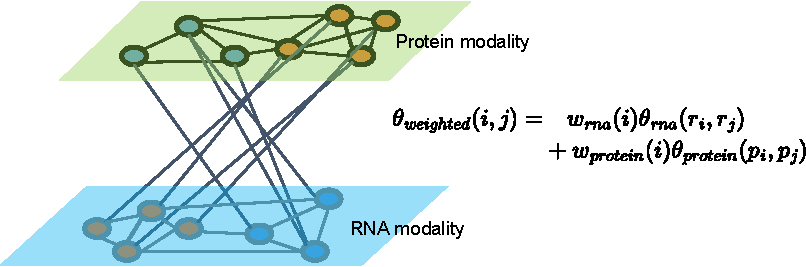
\includegraphics[width=0.60\textwidth]{Alg_WNN/fig}
  	\vspace{0.1cm}
  	\caption[Illustration of Seurat WNN integration competing method.]{\textbf{Illustration of Seurat WNN integration competing method.} Seurat weighted nearest neighbor(WNN) constructs a single unified representation across multiple modalities by initially creating k-nearest neighbor~(KNN) graphs for each modality based on the latent representation of each feature matrix. Subsequently, it calculates affinities using the exponential kernel between a cell and the average nearest neighbors for each modality. The latter is utilized to weigh cells in the unified representation. \emph{Source~\cite{hao2021seurat4}}~(modified to fit thesis format and/or clarify key points)
  }
  	\label{fig:Alg_WNN}
\end{figure}

  \item[Seurat WNN]
  Weighted nearest neighbor~(WNN)~\citep{hao2021seurat4}) constructs a single unified representation across multiple modalities. First, it creates k-nearest neighbor~(KNN) graphs for each modality based on the latent representation of each feature matrix. Next, it calculates affinities using the exponential kernel between a cell and the average NN for each modality. The latter is used to weigh cells. It finally calculated the weighted similarity between $cell_i$ and $cell_j$ as the dot product of $\textbf{w}_m(i)$ and $\theta(i,j)$,
  \begin{equation}
  	\theta_{weighted}(i,j)=\sum_{m} \textbf{w}_m(i)\theta(i,j)
  \end{equation}
  Where $\textbf{w}_m(i)$ is the weight of cell $i$ in modality $m$ and $\theta(i,j)$ denotes the affinity between cell $i$ and cell $j$ in modality $m$~(\fref{fig:Alg_WNN}).


  \item \textbf{Symphony Integration}
  Symphony~\citep{kang2021symphony} is a method to create single cell reference atlas for subsequent annotation of new single cell data sets. For a single case study with a multi-ome CITE-seq data, Symphony used canonical correlation analysis to find shared references. This simple procedure differs from MOJITOO in several ways: it does not use dimension reduction as input; it is not able to cope with more than 2 modalities and it uses the latent space of only one modality~(RNA) as shared space. Moreover, Symphony included the execution of batch correction with Harmony after the execution of CCA.

\end{description}


\subsubsection{Single Cell Multimodal Integration Objective}
Single-cell simultaneous modalities profiling is a nascent area, offering insights into biological processes and cellular heterogeneity. However, the complexity of different modalities' features and the growing library size present challenges, necessitating tools for integration In this thesis, we investigate the aspects with the flowing goals to develop a single cell multimodal integration method:

\begin{itemize}
	\item
	The objective is to develop an innovative computational method proficient in integrating more than two modalities with efficacy. The method should adeptly handle scenarios where modalities lack shared features and effectively address batch correction issues arising from diverse data batches. Furthermore, the method must yield a cohesive latent space suitable for clustering, data visualization, and subsequent analyses. Crucially, this latent space should be interpretable, facilitating the association of a component with the original feature count matrix. This interpretability enables a nuanced understanding of components, encompassing aspects such as gene expression and TF activity. Lastly, the methods should be computationally efficient to handle the increasingly larger single-cell library sizes.
	\item
	Establishing a comprehensive benchmarking framework for multimodal integration is imperative. All methods aferomentioned in \sref{background:sec2:integration} will be evaluated in \sref{chapter:MOJITOO_bench}. Acknowledging that ground truth labels~(cell type) may not infallibly represent actual biological facts due to manual cell annotation, it is crucial to devise a sophisticated set of benchmarking metrics. Beyond the clustering arrangement alignment with true labels, the benchmarking should encompass structural similarity evaluations between the shared latent space and each modality. Additionally, it should address the evolving levels of shared latent space distances among cells originating from the original modalities.

	\item
	We should curate diverse sets of simultaneous multimodal datasets for benchmarking, incorporating two datasets that simultaneously profile single-cell RNA sequencing~(scRNA) and single-cell Assay for Transposase-Accessible Chromatin sequencing~(scATAC), two datasets comprising scRNA and single-cell surface protein information, and two datasets involving all three prevalent types: scRNA, scATAC, and single cell surface protein. This comprehensive approach ensures a more equitable and robust benchmarking outcome.

	\item
	We should strive to interpret the components of the latent space using a dataset, gaining biological insights to determine whether it effectively captures cell type signals or signals related to cell fate differentiation. Additionally, we aim to interpret the latent space by associating it with the gene expression count matrix and epigenomic peak count matrix, selecting features to demonstrate the capabilities of our model.
\end{itemize}
\FloatBarrier %% step figure jump to the next subsection.

\subsection{Single Cell Multimodal Trajectory Inference}
We will present the computational challenge of trajectory inference for single-cell multimodal data, provide an overview of current methods developed in this field, and outline our goals to develop a method that addresses these challenges.

\subsubsection{Challenge of Single Cell Trajectory Inference}
\label{background:sec2:challenge_TI}
Computational trajectory analysis, which explores non-linear embeddings in the cellular space and algorithms to find paths or trees in these spaces, is quite popular in the analysis of single cells~\citep{wolf2019paga,chen2019stream,street2018slingshot,Lynch2022}. Despite the power of these approaches~\citep{saelens2019comparison}. There are still some challenges that need to be addressed:

\begin{figure}[!h]
	\centering
	\includegraphics[width=0.95\textwidth]{cell_differentiation/fig}
	\vspace{0.1cm}
	\caption[Hematopoiesis Cellular Differentiation]{\textbf{Hematopoiesis Cellular differentiation.} \textbf{A)} Hematopoiesis differentiation tree. Cell types are hematopoietic stem cell~(HSC), common myeloid progenitor~(CMP),  common lymphoid progenitor~(CLP), megakaryocyte–erythroid progenitor cell~(MEP), granulocyte-macrophage progenitor~(GMP), platelet~(Pla), erythrocyte~(Ery), granulocyte~(Gn), monocytes~(Mo), macrophages(M$\phi$), T cell~(T), B cell~(B) and Natural killer cell~(NK). \textbf{B)} GMP differentiation into two cell types~(Gn and Mo). GMP cells undergo differentiation into two distinct cell types, namely, granulocytes~(Gn) and monocytes~(Mo). During this differentiation process, specific regions of the chromatin become open, and different transcription factors bind to these regions, ultimately influencing the gene expression patterns that characterize these two cell types. \emph{Source:~\cite{costa2023dissecting}}~(modified to fit thesis format and/or clarify key points)}
	\label{fig:cell_differentiation}
\end{figure}

\begin{itemize}
	\item \textbf{Cell Differentiation in Biology:}
	The cell types in a multicellular organism become different from one another, as illustrated in \fref{fig:cell_differentiation}A, which shows a hematopoiesis differentiation tree. This cellular differentiation process is controlled by transcription factors~(TFs) binding to specific DNA regions called enhancers/promoters to recruit polymerases and modulate the expression of genes, eventually leading to the formation of different cell types~(\fref{fig:cell_differentiation}B)~\citep{costa2023dissecting}. Multimodal data with simultaneous epigenome and transcriptome information provide a better opportunity to explore this process. However, few trajectory inference methods make use of multimodal data to inspect cellular differentiation events.


	\item \textbf{Complexity of multi-branching trajectories:}
	For complex datasets, such as hematopoiesis~(\fref{fig:cell_differentiation}A), where cell differentiation leads to various immune cell types, monocytes, myeloid cells, and their subtypes, a method capable of capturing intricate differentiation processes is required. Unfortunately, many existing methods struggle to accurately capture the trajectory structure of such complex datasets.


	\item \textbf{Most approaches use low number of dimensions~($\geq3$) to fit trajectories:}
	As high-dimensional data cannot be naturally visualized, trajectories of single-cell data are typically represented in embeddings with only 2 to 3 dimensions. However, this approach necessitates the omission of high-dimensional information. To address this limitation, there is a need for methods that directly infer cell differentiation from high-dimensional embeddings.

	\item \textbf{Graph-based methods only use the information of nodes:}
	Methods such as Minimum Spanning Tree, ElPiGraph, or diffusion processes typically focus solely on cell position information, capturing only the relation between cells. These approaches neglect high-order graph features such as edges and triangles, which grasp the relationship between edges and triangles.

	\item \textbf{Few Methods are designed for multimodal data:}
	In the emerging field of single-cell multimodal analysis, many methods lack a comprehensive approach to trajectory inference across multiple modalities. While existing methods designed for single-cell transcriptomics, such as Slingshot and STREAM, can be applied to handle single-cell multimodal data, they often fall short in leveraging multimodal information for in-depth analyses, such as exploring gene regulation along a trajectory path using information from multiple modalities.
\end{itemize}
% a figure shows the feature type differences among different modalities

% a figure of single cell multimodal integration methods theory
\label{background:sec2:TI}
\subsubsection{Computational Methods for Trajectory Inference}
 The challenges highlighted in \sref{background:sec2:challenge_TI} regarding the trajectory inference of single-cell multimodal data present complexities in developing methods for handling multimodal data and data exhibiting intricate trajectory structures.

% table summarizing method
\begin{table}[!ht]
	\small
	\centering
	\begin{tabular}{llll}
		\toprule
		Name & Programming & Technique & Reference \\
		\midrule
    Celltree& R& LDA & \cite{duverle2016celltree}\\
    ElPigraph& Python/R & ElPigraph & \cite{albergante2020ElPiGraph}\\
    Monocle3 & R  & DDRTree/SimplePPT/L1Graph  & \cite{cao2019monocle3} \\
    MST & R & MST &  \cite{book2023mclust}\\
    PAGA	 & Python & kNN graph partitioning & \cite{wolf2019paga} \\
    pCreode & Python & d-kNN graph & \cite{herring2018pCreode} \\
		RaceID/StemID &  R & k-medoids clustering &  \cite{grun2016stemid} \\
    SLICE& R & MST & \cite{guo2017slice}\\
		Slingshot & R & MST & \cite{street2018slingshot}\\
		STREAM& Python & ElPigraph & \cite{chen2019stream}\\
    TSCAN & R & MST &  \cite{ji2016tscan}\\
		\bottomrule
	\end{tabular}
	\vspace{0.1cm}
	\caption[Overview of computational trajectory inference methods]{Overview of computational trajectory inference methods.}
	\label{tab:methods_ti_overview}
\end{table}
Next, we will discuss several published trajectory inference methods, All of them are top methods according to the dynverse trajectory inference evaluation system~\citep{saelens2019comparison} except STREAM a new method not yet implemented in dynverse. These methods can be broadly categorized into six groups. The first group involves methods utilizing a minimum spanning tree~(MST) to capture the backbone in the embeddings of a dataset~(e.g., TSCAN, slingshot, MST, slice). The second group includes methods like ElPiGraph, which leverages Elastic Principal Graphs to yield an explicit principal tree in data space~(ElPiGraph, STREAM). The third group employs topic model Latent Dirichlet Allocation~(LDA) from the natural language processing~(NLP) field for inference. The fourth group encompasses methods such as PAGA, using kNN graph partitioning, and pCreode, creating a d-kNN graph. The fifth group utilizes cluster distances for inference to derive the structure~(RaceID/StemID). The last method, Monocle3, seeks to create a principal graph on dimension reductions. These methods are summarized in \tref{tab:methods_ti_overview} illustrates the workflow of most of the methods.
\begin{description}

\begin{figure}[h!]
  	\centering
  	\includegraphics[width=0.95\textwidth]{TI_comparison/fig}
  	\vspace{0.1cm}
  	\caption[Illustration of TI methods schematic.]{\textbf{Illustration of TI methods schematic.} celltree, elpigraph, monocle3, pCreode, StemID, SLICE, slingshot, STREAM and TSCAN.\emph{Source:~\cite{duverle2016celltree,albergante2020ElPiGraph,cao2019monocle3,herring2018pCreode,grun2016stemid,guo2017slice,street2018slingshot,chen2019stream,ji2016tscan}}~(modified to fit thesis format and/or clarify key points)
  	}
  	\label{fig:TI_comparison}
\end{figure}


\begin{figure}[h!]
  	\centering
  	\includegraphics[width=0.55\textwidth]{TI_Alg_celltree/fig}
  	\vspace{0.1cm}
  	\caption[Illustration of TI method Celltree schematic.]{\textbf{Illustration of TI method Celltree schematic.} Celltree use myoblast data as example. Backbone tree obtained from the dataset of differentiating myoblasts with cellTree. Larger nodes indicate backbone cells~(selected representatives), whereas smaller nodes represent cells that only show slight variations from the backbone cell they are attached to. Cell nodes have been coloured according to \textbf{A} their sampling time~(in hours from the start of the differentiation process) and \textbf{B} their distribution over topics. \emph{Source:~\cite{duverle2016celltree}}~(modified to fit thesis format and/or clarify key points)
  	}
  	\label{fig:TI_Alg_celltree}
\end{figure}
  \item[Celltree]
  To identify and utilize group structure, Celltree~\citep{duverle2016celltree} adapts a natural language processing~(NLP) statistical approach known as Latent Dirichlet Allocation~(LDA) to build a topic model. By comparing the different per-cell topic histograms, celltree can evaluate their similarity and infer complex hierarchical structures. By looking at the topics themselves, one can obtain useful biological insights into the gene sets characterizing the different stages of that hierarchy. Based on this lower-dimensional model, it constructs a visual representation of the cell population. finally, Celltree introduces ``backbone trees'' to easily visualize cells along complex differentiation paths~(\fref{fig:TI_Alg_celltree}).
  

\begin{figure}[h!]
  	\centering
  	\includegraphics[width=0.85\textwidth]{TI_Alg_ElPiGraph/fig}
  	\vspace{0.1cm}
  	\caption[Illustration of TI method ElPiGraph schematic.]{\textbf{Illustration of TI method ElPiGraph schematic.} Schematic workflow of the ElPiGraph method. On the left, the construction of the elastic graph starts by defining the initial graph topology and embedding it into the data space. The graph structure is fitted to the data, minimizing the mean square error regularized by the elastic energy. The elastic energy includes a term reflecting the overall stretching of the graph~(symbolically shown as contractive red springs) and a term reflecting the overall bending of the graph branches and the harmonicity of branching points~(shown as repulsive green springs). In the middle, ElPiGraph explores a large region of the structural space by exhaustively applying a set of graph rewriting rules~(graph grammars) and selecting, at each step, the structure leading to the minimum overall energy of the graph embedding. \emph{Source:~\cite{cao2019monocle3}}~(modified to fit thesis format and/or clarify key points)
  	}
  	\label{fig:TI_Alg_ElPiGraph}
\end{figure}

  \item[ElPiGraph]
  Elastic Principal Graphs~(ElPiGraphs)~\citep{albergante2020ElPiGraph} serve as structured approximators for data, comprising vertices connected by edges. These vertices are embedded into the data space, minimizing mean squared distance~(MSD) to data points. Notably, ElPiGraphs differ from unstructured k-means by incorporating edges to define an elastic energy term. This term, coupled with MSD, penalizes edge stretching and branch bending. ElPiGraph employs a topological grammar for optimal graph structure determination, building on a core algorithm initially introduced and tested in earlier publications~\citep{gorban2007topological}. In essence, an elastic principal graph is an undirected graph in multidimensional space, optimizing data approximation and graph elastic energy. Key parameters, including trimming radius~($R_0$), edge elasticity~($\lambda$), star bending elasticity~($\mu$), and a complexity control coefficient~($\alpha$), guide the optimization process. ElPiGraph achieves efficient minimization by employing a quadratic problem-solving approach for vertex coordinates. It uses topological grammars, exploring diverse graph structures, and iteratively refining configurations until specified conditions are met. Finally, ElPiGraph yields an explicit principal tree in data space, facilitating independent study or mapping data onto the tree for analysis in intrinsic coordinates~(\fref{fig:TI_Alg_ElPiGraph}).


\begin{figure}[h!]
  	\centering
  	\includegraphics[width=0.90\textwidth]{TI_Alg_Monocle3/fig}
  	\vspace{0.1cm}
  	\caption[Illustration of TI method Monocle3 schematic.]{\textbf{Illustration of TI method Monocle3 schematic.} Monocle3 aims to learn a principal graph by using SimplePPT, DDRTree or L1Graph, with which, each cell is projected onto the graph. By selecting the starting points on the graph, Monocle measures the distance from these points to each cell, determining a cell's pseudotime as the distance to the closest starting point on the graph. \emph{Source:~\cite{cao2019monocle3}}~(modified to fit thesis format and/or clarify key points)
  	}
  	\label{fig:TI_Alg_Monocle3}
\end{figure}

  \item[Monocle3]
  Monocle3 undergoes a comprehensive five-step process in single-cell dataset analysis~\citep{cao2019monocle3}. Firstly, it normalizes and pre-processes data, addressing technical variations. The second step involves reducing dimensionality by projecting cells onto the top 50 principal components, with options for further reduction using t-SNE or UMAP. In the third step, Monocle 3 clusters and partitions cells, recognizing disconnected trajectories or ``supergroups" that capture diverse cellular responses. Subsequently, it learns a principal graph, utilizing methods like DDRTree, SimplePPT, or L1Graph, accommodating tree-like or looped trajectories. Finally, Monocle 3 conducts differential expression analysis and visualization for exploring gene dynamics across clusters and trajectories with sophisticated testing methods~(\fref{fig:TI_Alg_Monocle3}).

\begin{figure}[h!]
  	\centering
  	\includegraphics[width=0.85\textwidth]{TI_Alg_PAGA/fig}
  	\vspace{0.1cm}
  	\caption[Illustration of TI method PAGA schematic.]{\textbf{Illustration of TI method PAGA schematic.}
  	PAGA uses partition-based graph abstraction generating a topology-preserving map of single cells. It creates a kNN graph and partitions it using the Louvain algorithm at a desired resolution where partitions represent groups of connected cells. Next, A PAGA graph is obtained by associating a node with each partition and connecting each node by weighted edges that represent a statistical measure of connectivity between partitions. PAGA graphs reveal the denoised topology of the data at a chosen resolution by discarding low-weight edges. \emph{Source:~\cite{wolf2019paga}}~(modified to fit thesis format and/or clarify key points)
  	}
  	\label{fig:TI_Alg_PAGA}
\end{figure}

  \item[PAGA]
  Probabilistic Approximate Graph Abstraction~(PAGA) uses partition-based graph abstraction generating a topology-preserving map of single cells~\citep{wolf2019paga}. High-dimensional gene expression data is represented as a kNN graph by choosing a suitable low-dimensional representation and an associated distance metric for computing neighborhood relations. The kNN graph is partitioned using the Louvain algorithm at a desired resolution where partitions represent groups of connected cells. A PAGA graph is obtained by associating a node with each partition and connecting each node by weighted edges that represent a statistical measure of connectivity between partitions. By discarding spurious edges with low weights, PAGA graphs reveal the denoised topology of the data at a chosen resolution and reveal its connected and disconnected regions. Combining high-confidence paths in the PAGA graph with a random-walk-based distance measure on the single-cell graph, PAGA orders cells within each partition according to their distance from a root cell. A PAGA path then averages all single-cell paths that pass through the corresponding groups of cells. This allows to trace gene expression changes along complex trajectories at single-cell resolution~(\fref{fig:TI_Alg_PAGA}).

\begin{figure}[h!]
  	\centering
  	\includegraphics[width=0.65\textwidth]{TI_Alg_pCreode/fig}
  	\vspace{0.1cm}
  	\caption[Illustration of TI method pCreode schematic.]{\textbf{Illustration of TI method pCreode schematic.} pCreode carries out 6 steps to infer a trajectory. It creates a density-based k-nearest neighbor~(d-kNN) network and constructs topology with a hierarchical placement strategy of cells on path nodes between end-state clusters. Next, it iteratively redoes the arrangement of the topology according to the neighborhood cell densities. \emph{Source:~\cite{herring2018pCreode}}~(modified to fit thesis format and/or clarify key points)
  	}
  	\label{fig:TI_Alg_pCreode}
\end{figure}

  \item[pCreode]
  %pCreode infer a trajactory for single-cell data through 7 steps:~(i) Input single-cell expression data.~(ii) Density-normalized representation after down-sampling the original dataset. Overlay shows density post down-sampling.~(iii) Density-based k-nearest neighbor~(d-kNN) network from down-sampled data. Overlay represents closeness centrality, a surrogate for cell state.~(iv) K-means clustering identifies end-states based on low closeness values~($<$mean). The number of clusters is doubled for rare cell types.~(v) Topology constructed with a hierarchical placement strategy between end-states, allowing data points along an ancestral continuum. Overlay shows original cell density.~(vi) Aligned topology~(red) achieved through iterative assignment and repositioning of path nodes using neighborhood cell densities.~(vii) Representative topology extracted using p-Creode scoring from an ensemble of N topologies, with node size indicating the original cell density.

  pCreode infer a trajactory for single-cell data through 6 steps~\citep{herring2018pCreode}. 1) Conducts density-dependent down-sampling to normalize the representation of both rare and overrepresented cell states; 2) Constructs a density-based k-nearest neighbor~(d-kNN) network using the down-sampled data; 3) Automatically distinguishes end-states from transition states by employing K-means clustering and assessing silhouette scores for cells with low closeness values~(< mean); 4) Establishes topology through a hierarchical placement strategy, positioning cells on path nodes between end-states; 5) Aligns topology with maximal consensus through an iterative process involving the assignment and repositioning of path nodes based on neighborhood cell densities; 6) Develops a scoring metric within pCreode to compare dissimilarities between topologies facilitating the selection of the most representative graph for visualization purposes~(\fref{fig:TI_Alg_pCreode}).

  \begin{figure}[h!]
  	\centering
  	\includegraphics[width=0.55\textwidth]{TI_Alg_StemID/fig}
  	\vspace{0.1cm}
  	\caption[Illustration of TI method RaceID/StemID schematic.]{\textbf{Illustration of TI method RaceID/StemID schematic.}
  	RaceID/StemID initially conducts clustering using RaceID2~(k-medoids clustering). Next, it infers putative differentiation trajectories by linking the medoids of two clusters, defining the possible topology of the lineage tree. It then assigns each cell to an inter-cluster link by selecting the longest projection. \emph{Source:~\cite{albergante2020ElPiGraph}}~(modified to fit thesis format and/or clarify key points)
  	}
  	\label{fig:TI_Alg_StemID}
  \end{figure}

  \item[RaceID/StemID]
  StemID~\citep{grun2016stemid} uses RaceID~\citep{grun2015raceid}, an advanced version of RaceID to perform clustering. Next, to address the challenge of determining branching points in systems with multiple cell lineages for building the lineage tree with guided topology StemID predefines the tree's structure by allowing potential differentiation trajectories between pairs of clusters. Each trajectory links the medoids of two clusters, and collectively, these inter-cluster links determine the possible lineage tree's topology. To mitigate technical noise and computational load, It initially reduces input space dimensionality, emphasizing maximal preservation of point-to-point distances. Next, it assigns each cell to its likely position on a single inter-cluster link based on the projection of the vector connecting a cluster's medoid to one of its cells onto links with other clusters' medoids. By normalizing link lengths and identifying densely populated links, StemID discerns potential differentiation trajectories~(\fref{fig:TI_Alg_StemID}).

\begin{figure}[h!]
  	\centering
  	\includegraphics[width=0.65\textwidth]{TI_Alg_SLICE/fig}
  	\vspace{0.1cm}
  	\caption[Illustration of TI method SLICE schematic.]{\textbf{Illustration of TI method SLICE schematic.}
  	SLICE first measures cell differentiation states based on the calculation of single-cell entropy (scEntropy) and then predicts cell differentiation trajectories by ordering single cells according to their scEntropy-derived differentiation states. \emph{Source:~\cite{guo2017slice}}~(modified to fit thesis format and/or clarify key points)
  	}
  	\label{fig:TI_Alg_SLICE}
\end{figure}

  \item[SLICE]
  Single Cell Lineage Inference Using Cell Expression Similarity and Entropy~(SLICE)~\citep{guo2017slice} comprises two main functions: quantitatively assessing cell differentiation state through single-cell entropy and reconstructing single-cell lineages in silico. The calculation of single-cell entropy~(scEntropy) involves computing the expected value for each cell, representing the uncertainty in cellular functions activation based on gene expression patterns. The scEntropy is utilized to measure the differentiation state of individual cells. Stable states are identified within scRNA-seq datasets using clustering or graph-based methods, considering the scEntropy of each cell. SLICE then constructs a lineage model by inferring a directed minimum spanning tree among stable states, reflecting differentiation trajectories. The reconstruction of cell transitional paths involves either a shortest-path approach or a principal curve-based approach, revealing the dynamics of gene expression during differentiation. Lineage-dependent differentially expressed genes are identified based on smoothed expression profiles, and temporal gene expression patterns are unveiled through clustering analysis~(\fref{fig:TI_Alg_SLICE}).

\begin{figure}[h!]
  	\centering
  	\includegraphics[width=0.8\textwidth]{TI_Alg_slingshot/fig}
  	\vspace{0.1cm}
  	\caption[Illustration of TI method Slingshot schematic.]{\textbf{illustration of TI method Slingshot schematic.}
  	Firstly, a Minimum Spanning Tree~(MST) is constructed on the clusters to determine the number and rough shape of lineages. Following that, simultaneous principal curves are employed to obtain smooth representations of each lineage. \emph{Source:~\cite{street2018slingshot}}~(modified to fit thesis format and/or clarify key points)
  	}
  	\label{fig:TI_Alg_slingshot}
\end{figure}

  \item[Slingshot]
  Slingshot~\citep{street2018slingshot} infers a trajectory of datasets with multiple branches by comprising two distinct stages: 1) Global Lineage Structure Inference. In this stage slingshot employs Minimum Spanning Tree~(MST) on clustered data points to infer the overall lineage structure. By utilizing a cluster-based MST, Slingshot stably identifies essential elements such as the number of lineages and their branching points. 2) Pseudotime Inference for Individual Lineages. In the second stage, Slingshot introduces a novel approach known as simultaneous principal curves. This method fittingly applies smooth branching curves to the identified lineages, translating the knowledge of the global lineage structure into reliable estimates of cell-level pseudotime variables for each lineage~(\fref{fig:TI_Alg_slingshot}).

\begin{figure}[h!]
  	\centering
  	\includegraphics[width=0.95\textwidth]{TI_Alg_STREAM/fig}
  	\vspace{0.1cm}
  	\caption[Illustration of TI method STREAM schematic.]{\textbf{Illustration of TI method STREAM schematic.} STREAM first selection of informative genes from a single cell count matrix, followed by dimensional reduction. Next, it learns and fits simultaneous tree structure by ElPiGraph. The optimal structure is selected based on the elastic energy minimization among a set of candidate structures that are constructed every time a tree node is added. The final tree is interpreted as a set of connected curves representing different trajectories. \emph{Source:~\cite{chen2019stream}}~(modified to fit thesis format and/or clarify key points)
  	}
  	\label{fig:TI_Alg_STREAM}
\end{figure}

  \item[STREAM]
  Single-cell Trajectories Reconstruction, Exploration And Mapping~(STREAM) takes a single-cell gene expression matrix as input~\citep{chen2019stream}. Next, it performs three main steps: selection of informative genes, dimensionality reduction, and simultaneous tree structure learning and fitting by ElPiGraph. The optimal structure is selected based on the elastic energy minimization among a set of candidate structures that are constructed every time a tree node is added. The final tree is interpreted as a set of connected curves representing different trajectories~(\fref{fig:TI_Alg_STREAM}).

\begin{figure}[h!]
  	\centering
  	\includegraphics[width=0.65\textwidth]{TI_Alg_TSCAN/fig}
  	\vspace{0.1cm}
  	\caption[Illustration of TI method TSCAN schematic.]{\textbf{Illustration of TI method TSCAN schematic.}
  	TSCAN initially constructs a cluster-based Minimum Spanning Tree~(MST) with multiple paths. Next, TSCAN orders cells along each path by projecting them onto the tree edges. \emph{Source:~\cite{ji2016tscan}}~(modified to fit thesis format and/or clarify key points)
  	}
  	\label{fig:TI_Alg_TSCAN}
\end{figure}

  \item[TSCAN]
  pseudo-Time reconstruction in Single-Cell RNA-seq ANalysis~(TSCAN)~\citep{ji2016tscan} first uses PCA to reduce the dimensionality. It uses the clustering algorithm Mclust to model the datasets as a mixture of normal distributions, to cluster the cells while automatically determining the number of clusters using the Bayesian information criterion. Next, It infers a trajectory by identifying the longest connected path through the Minimum Spanning Tree~(MST) tree, which is created through the cluster center. Finally, all the cells are projected to the nearest point on the trajectory, creating the final ordering. TSCAN automatically determines both start and end cell clusters without prior gene dimension filtering. However, slight changes in center locations can significantly impact the identified trajectory~(\fref{fig:TI_Alg_TSCAN}).


\end{description}

%\subsubsection{Celltree}
%\subsubsection{ElPiGraph}
%\subsubsection{Monocle3}
%\subsubsection{PAGA}
%\subsubsection{pCreode}
%\subsubsection{RaceID/StemID}
%\subsubsection{SLICE}
%\subsubsection{Slingshot}
%\subsubsection{STREAM}
%The Elastic principal graph:
%\begin{equation}
%	\begin{aligned}
%& U^{\phi}(X, G) = \frac{1}{|x|}\sum_{j=1}^{|V|} \sum_{i:P(i)=j} \min \left(\left\|X_i - \phi(V_j)^2, R_0^2\right\|\right) \\
%&\quad + \sum_{E^{(i)}}[\lambda + \alpha(\max(2, \deg(E^{(i)}(0))) - 2)](\phi(E^{(i)}(0)) - \phi(E^{(i)}(1)))^2 \\
%&\quad + \mu \sum_{S^{(j)}} \left(\phi(S^{(j)(0)}) - \frac{1}{\deg (S^{(j)(0)})} \sum_{i = 1}^{\deg (S^{(j)(0)})}\right)^2
%	\end{aligned}
%\end{equation}
%where $X=\{X_i\}, i = 1\cdots|X|$ is a set of points, $E^{(i)}(0)$ and $E^{(i)(1)}$ denotes the two vertices of a graph edge $E^{(i)}$, and $S^{(j)(0)},\cdots S^{(j)}(k)$ denote the vertices of the a star $S^{(j)}$ in the graph. $P(i)$ is a data point partitioning function associating each data point $X_i$ to the closest vertex index that $P(i) = \arg\min_{j=1\cdots |V|}$. $phi{V_j}$ is the mapping function that $\phi: V \rightarrow R^{m}$, which defines a position of $j$th graph vertex in the multidimensional space of data. Finally, $R_0$ is the trimming radius such that points further than $R_0$ from any nodes don't contribute to the optimization of the graph, and $\lambda$ is the edge stretching elasticity modulo regularizing the total length of the graph, and $\alpha$ is a coefficient to control the complexity of the graph. $\mu$ is the star bending elasticity that controls the smoothness of the graph.
%\subsubsection{TSCAN}
%\subsubsection{Slicer}
%Slicer is a KNN-based trajectory inference method that utilizes alpha-hull to estimate the k parameter for locally linear embedding dimensionality reduction. First, Slicer computes a KNN graph from locally linear embedding, next it finds the most “extreme” cells in the graph. The user needs to specify a starting cell from extreme cells, Slicer then find the shortest path to all other cells. Next, the geodesic entropy is used to find branches; high values indicate the existence of a branching point.

\subsubsection{Single Cell Multimodal Trajectory Inference Objective}
Single-cell simultaneous modalities profiling is a nascent area, offering insights into biological processes and cellular heterogeneity. necessitating tools for trajectory inference. In this thesis, we also investigate the aspect of developing a trajectory inference method for single cell multimodal data:
\begin{itemize}
	\item
	The aim is to develop a new computational method to infer a trajectory tree effectively capturing cell differentiation events. The method should adeptly handle complex tree structure datasets, delving deeper into the graph structure by considering not only the relations between nodes and edges but also the edges and triangles within a graph. Furthermore, the method should be applicable to single-cell multimodal data.

	\item
	The method should offer an elegant visualization of the inferred trajectory tree. Additionally, it should provide functions to perform branch differentiation, enabling the identification of significantly expressed marker genes or marker TF activities for specific comparisons. To facilitate single-cell multimodal analysis, the method should also incorporate an approach to correlate different features, such as gene expression and transcription factor activity, along a trajectory branch.

	\item
	To evaluate its efficacy, we will generate high-dimensional simulated data with varying tree branches, ranging from small to large, to assess the model's capability to capture intricate tree structures. Benchmarking will be performed using the dynverse Trajectory Inference evaluation framework, comparing our method with top-ranked methods.

	\item
	All methods aferomentioned~\sref{background:sec2:TI} will be evaluate in \sref{chapter:PHLOWER_bench} The evaluation of the methods should include an examination of the topological similarity between the inferred trajectory and the ground truth. Furthermore, it should evaluate the accuracy of cell branch allocation and scrutinize the order of cells within each branch, as well as the accuracy of branching point allocation.

	\item The application of our method to in-house single-cell multimodal data involves implementing the 10$\times$ multiome protocol on kidney organoid data at four distinct time points: day 5, day 12, day 19, and day 25. We aim to assess the capability of our method in capturing cell differentiation. Additionally, we plan to uncover insights by exploring the trajectories of our model through statistical differentiation of branches and correlation analyses between genes and transcription factor(TF) activities. To further validate our findings, we intend to conduct TF knockouts and assess their impact on preventing incorrect cell type differentiation.

\end{itemize}

% table of single cell trajectory inference methods

% a figure of single cell trajectory inference methods theory
\section{Discussion}
\label{background:Discussion}
In this chapter, we initially provided an overview of DNA structure and gene regulatory processes. Subsequently, we introduced the profiling techniques for single-cell transcriptome, epigenome, and proteome, including simultaneous profiling protocols. We then delved into the computational analyses associated with these modalities. Subsequently, we directed our focus towards computational analysis methods for single-cell multimodal data. We addressed the challenges posed by two critical analyses: single-cell multimodal integration and trajectory inference. We discussed the related work and outlined our objectives for tackling these tasks.
